%% Ternary complex model
%% FigThreeStateDimer.tex
%% Unused packages and definitions removed; TikZ/PGFPlots source formatted.

\documentclass[tikz,margin=2mm]{standalone}
\usetikzlibrary{arrows}

\def\b{\mathsf{b}}
\def\c{\mathsf{c}}

\def\kappab{\kappa_{\b}}
\def\kappac{\kappa_{\c}}

\def\kappabp{\kappa_{\underline{\b}}}
\def\kappacp{\kappa_{\underline{\c}}}

\def\etabb{\eta_{\b\b}}
\def\etabc{\eta_{\b\c}}
\def\etacc{\eta_{\c\c}}

\def\etabbp{\eta_{\b\underline{\b}}}
\def\etacbp{\eta_{\c\underline{\b}}}
\def\etabcp{\eta_{\b\underline{\c}}}
\def\etaccp{\eta_{\c\underline{\c}}}

\def \half {\frac{1}{2}}

\begin{document}

\tikzset{every node/.style={minimum size=0.2cm,inner sep=2pt,outer sep=3pt}}
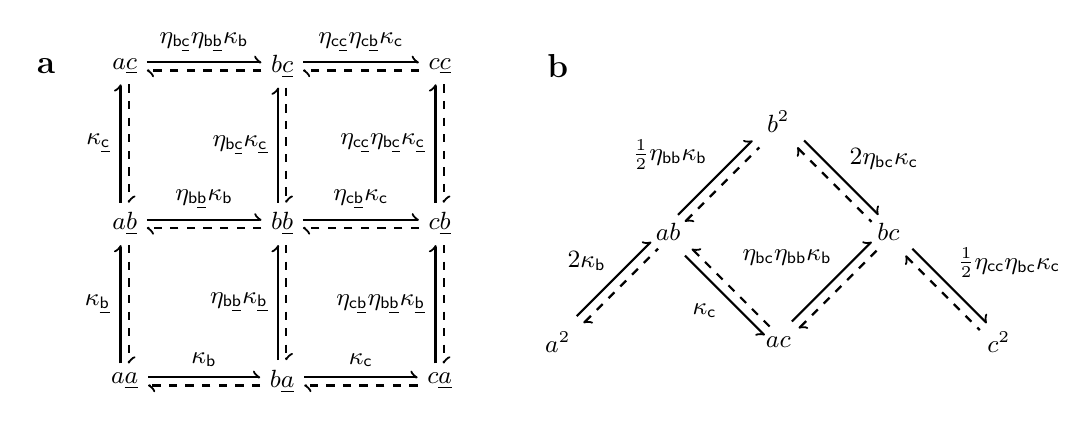
\begin{tikzpicture}[node distance=2.0cm,>=latex',font=\small]
    \begin{scope}[xshift=1cm]
        %\draw (-1.2,0) node (LEFTAP) {$\underline{a}$};
        %\node[above of = LEFTAP] (LEFTBP) {$\underline{b}$};
        %\node[above of = LEFTBP] (LEFTCP) {$\underline{c}$};

        %\draw (0,-1.2) node (BOTTOMA) {$a$};
        %\node[right of = BOTTOMA] (BOTTOMB) {$b$};
        %\node[right of = BOTTOMB] (BOTTOMC) {$c$};

        \draw (0,0) node (AAP) {$a\underline{a}$};
        \node[above of=AAP] (ABP) {$a\underline{b}$};
        \node[above of=ABP] (ACP) {$a\underline{c}$};

        \node[right of=AAP] (BAP) {$b\underline{a}$};
        \node[right of=ABP] (BBP) {$b\underline{b}$};
        \node[right of=ACP] (BCP) {$b\underline{c}$};

        \node[right of=BAP] (CAP) {$c\underline{a}$};
        \node[right of=BBP] (CBP) {$c\underline{b}$};
        \node[right of=BCP] (CCP) {$c\underline{c}$};

        %\draw [-left to,thick,transform canvas={xshift=-1.5pt}] (LEFTAP) to node[left] {$\kappa_{ab}^\prime$} (LEFTBP);
        %\draw [dashed,-left to,thick,transform canvas={xshift=1.5pt}] (LEFTBP) to (LEFTAP);

        %\draw [-left to,thick,transform canvas={xshift=-1.5pt}] (LEFTBP) to node[left] {$\kappa_{bc}^\prime$} (LEFTCP);
        %\draw [dashed,-left to,thick,transform canvas={xshift=1.5pt}] (LEFTCP) to (LEFTBP);

        \draw[-left to,thick,transform canvas={xshift=-1.5pt}] (AAP) to node[left] {$\kappabp$} (ABP);
        \draw[dashed,-left to,thick,transform canvas={xshift=1.5pt}] (ABP) to (AAP);

        \draw[-left to,thick,transform canvas={xshift=-1.5pt}] (ABP) to node[left] {$\kappacp$} (ACP);
        \draw[dashed,-left to,thick,transform canvas={xshift=1.5pt}] (ACP) to (ABP);

        \draw[-left to,thick,transform canvas={xshift=-1.5pt}] (BAP) to node[left] {$\etabbp \kappabp$} (BBP);
        \draw[dashed,-left to,thick,transform canvas={xshift=1.5pt}] (BBP) to (BAP);

        \draw[-left to,thick,transform canvas={xshift=-1.5pt}] (BBP) to node[left] {$\etabcp \kappacp$} (BCP);
        \draw[dashed,-left to,thick,transform canvas={xshift=1.5pt}] (BCP) to (BBP);

        \draw[-left to,thick,transform canvas={xshift=-1.5pt}] (CAP) to node[left] {$\etacbp \etabbp \kappabp$} (CBP);
        \draw[dashed,-left to,thick,transform canvas={xshift=1.5pt}] (CBP) to (CAP);

        \draw[-left to,thick,transform canvas={xshift=-1.5pt}] (CBP) to node[left] {$\etaccp \etabcp \kappacp$} (CCP);
        \draw[dashed,-left to,thick,transform canvas={xshift=1.5pt}] (CCP) to (CBP);

        %\draw [-left to,thick,transform canvas={yshift=1.5pt}] (BOTTOMA) to node[above] {$\kappa_{ab}$} (BOTTOMB);
        %\draw [dashed,-left to,thick,transform canvas={yshift=-1.5pt}] (BOTTOMB)to (BOTTOMA);

        %\draw [-left to,thick,transform canvas={yshift=1.5pt}] (BOTTOMB) to node[above] {$\kappa_{bc}$} (BOTTOMC);
        %\draw [dashed,-left to,thick,transform canvas={yshift=-1.5pt}] (BOTTOMC)to (BOTTOMB);

        \draw[-left to,thick,transform canvas={yshift=1.5pt}] (AAP) to node[above] {$\kappab$} (BAP);
        \draw[dashed,-left to,thick,transform canvas={yshift=-1.5pt}] (BAP)to (AAP);

        \draw[-left to,thick,transform canvas={yshift=1.5pt}] (BAP) to node[above] {$\kappac$} (CAP);
        \draw[dashed,-left to,thick,transform canvas={yshift=-1.5pt}] (CAP)to (BAP);

        \draw[-left to,thick,transform canvas={yshift=1.5pt}] (ABP) to node[above] {$\etabbp \kappab$} (BBP);
        \draw[dashed,-left to,thick,transform canvas={yshift=-1.5pt}] (BBP)to (ABP);

        \draw[-left to,thick,transform canvas={yshift=1.5pt}] (BBP) to node[above] {$\etacbp \kappac$} (CBP);
        \draw[dashed,-left to,thick,transform canvas={yshift=-1.5pt}] (CBP)to (BBP);

        \draw[-left to,thick,transform canvas={yshift=1.5pt}] (ACP) to node[above] {$\etabcp \etabbp \kappab$} (BCP);
        \draw[dashed,-left to,thick,transform canvas={yshift=-1.5pt}] (BCP)to (ACP);

        \draw[-left to,thick,transform canvas={yshift=1.5pt}] (BCP) to node[above] {$\etaccp \etacbp \kappac$} (CCP);
        \draw[dashed,-left to,thick,transform canvas={yshift=-1.5pt}] (CCP)to (BCP);
    \end{scope}

    %\begin{scope}[xshift=2.8cm,yshift=-1.3cm]
        %\draw[|-to,line width=5pt,gray!20,bend left=0] (0,1) to (0,0);
        %\end{scope}

    \begin{scope}[xshift=6.5cm,yshift=0.5cm,scale=0.7,style=thick,shorten >=0pt,shorten <=0pt,inner sep=1pt,outer sep=2pt]
        \def\rr{1}
        \draw (0,0) node (A2) {$a^2$};
        \draw (2,2*\rr) node (AB) {$ab$};
        \draw (4,4*\rr) node (B2) {$b^2$};
        \draw (4,0) node (AC) {$ac$};
        \draw (6,2*\rr) node (BC) {$bc$};
        \draw (8,0) node (C2) {$c^2$};

        % 2\kappa_b^{(a)}=
        \draw[-left to,thick,transform canvas={yshift=2.5pt}] (A2) to node[midway,above left] {$2\kappab$} (AB);
        \draw[dashed,left to-,thick,transform canvas={xshift=2.5pt}] (A2) to (AB);

        % \half\kappa_b^{(b)} =
        \draw[-left to,thick,transform canvas={xshift=-2.5pt}] (AB) to node[midway,above left] {$ \half\etabb \kappab$} (B2);
        \draw[dashed,left to-,thick,transform canvas={yshift=-2.5pt}] (AB) to (B2);

        % \kappa_b^{(c)}=
        \draw[-left to,thick,transform canvas={yshift=2.5pt}] (AC) to node[midway,above left,xshift=3pt,yshift=3pt] (ETATWO) {$\etabc \etabb \kappab$} (BC);
        \draw[dashed,left to-,thick,transform canvas={xshift=2.5pt}] (AC) to (BC);

        % 2\kappa_c^{(b)}=
        \draw[-left to,thick,transform canvas={xshift=2.5pt}] (B2) to node[midway,above right]  {$2\etabc\kappac$} (BC);
        \draw[dashed,left to-,thick,transform canvas={yshift=-2.5pt}] (B2) to (BC);

        % \half\kappa_c^{(c)}=
        \draw[-left to,thick,transform canvas={xshift=2.5pt}] (BC) to  node[midway,above right] {$\half\etacc\etabc\kappac $} (C2);
        \draw[dashed,left to-,thick,transform canvas={yshift=-2.5pt}] (BC) to (C2);

        % \kappa_c^{(a)}=
        \draw[dashed,right to-,thick,transform canvas={xshift=2.5pt}] (AB) to  (AC);
        \draw[-right to,thick,transform canvas={yshift=-2.5pt}] (AB) to node[midway,below left,xshift=0pt,yshift=0pt]  {$\kappac$} (AC);
    \end{scope}

    \def\height{4}
    \def\left{0}
    \draw (\left,\height) node[font=\large] {{\bf a}};
    \draw (\left+6.5,\height) node[font=\large] {{\bf b}};

    %\pgfresetboundingbox
    %\path (-0.2,-4.5) -- (6.5,-4.5) -- (6.5,5) -- (-0.2,5) -- cycle;

\end{tikzpicture}

\end{document}

